\section{保险丝}\label{sec:11-3}

照明电路里的每条电线都有规定的最大电流强度,如果通过的电流超过这个规定的最大值,
产生的热量会使电线的绝缘皮烧坏,甚至引起火灾。

引起电线中的电流超过规定值的原因,可能是电线连接的用电器的总功率过大,
例如私自连入了大功率的电炉;还可能是发生了短路。
所谓短路就是电流没有经过用电器而直接构成回路。
例如,在装修电灯时不细心,使两根电源线直接连通;电线绝缘皮被刮破,使两根电源线连通;
电线和用电器使用年久,绝缘破损或老化等等。发生短路时,电路中的电阻很小,所以电流强度很大。

避免电流超过电线规定值引起火灾的最好方法,是在电流增大到危险程度以前自动切断电路;
串联在电路里的保险丝就起这种作用。

家庭照明电路里的保险丝是由电阻率比较大而熔点较低的铅锑合金制成的。
它的保护作用可以从图 \ref{fig:11-5} 所示的实验看出来。
在 $C$、$D$ 之间接上保险丝,电路的其他部分用电线连接好。
当接上电源时,电灯正常发光,保险丝不熔断;
然后断开电源,在 $B$、$D$ 之间连上一根导线,造成短路。
再接上电源时,保险丝立即熔断,使电路断开,从而避免了电线烧坏。

\begin{figure}[htbp]
    \centering
    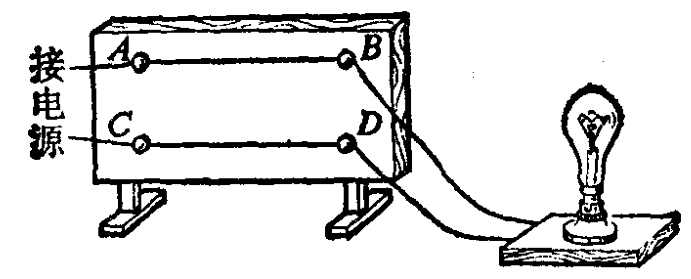
\includegraphics[width=0.6\textwidth]{../pic/czwl2-ch11-5}
    \caption{}\label{fig:11-5}
\end{figure}

保险丝的规格常用它的额定电流表示。
当通过的电流小于或等于保险丝的额定电流时,保险丝能正常通电。
如果电流超过它的额定电流达到它的熔断电流,它就迅速熔断。
不同材料、不同粗细的保险丝的额定电流不同。
下面的表列出了常用保险丝的额定电流和熔断电流。

% 下表中,为了实现让数字按小数点对齐,需要加载 siunitx 包,使用其中的 Q[si ...] 功能。
% 但这有一个问题,表头中的文字必须使用 {{{ }}} 括起来。括起来后,就不支持使用 \\ 实现换行。
% 所以,下`面的代码中,通过将表头拆成两行的方式规避了这一问题。
\begin{table}[htbp]
    \centering
    \caption*{\textbf{常用保险丝规格} \\(铅不少于 $98\%$,锑 0.3 ~ $1.5\%$,杂质不多于 $1.5\%$)}
    \begin{tblr}{
        colspec={Q[si={table-format=1.2},c]Q[si={table-format=3.2},c]Q[si={table-format=1.1},c]
               ||Q[si={table-format=1.2},c]Q[si={table-format=2.2},c]Q[si={table-format=2.1},c]},
        hline{1,3,13} = {1pt, solid},
        vline{1, 7} = {1pt, solid},
        vlines,
    }
        {{{直径}}} & {{{额定电流}}} & {{{熔断电流}}} & {{{直径}}} & {{{额定电流}}} & {{{熔断电流}}} \\
        {{{(毫米)}}} & {{{(安培)}}} & {{{(安培)}}} & {{{(毫米)}}} & {{{(安培)}}} & {{{(安培)}}}  \\
        0.28 & 1    & 2   & 0.81 & 3.75 & 7.5 \\
        0.32 & 1.1  & 2.2 & 0.98 & 5    & 10 \\
        0.35 & 1.25 & 2.5 & 1.02 & 6    & 12 \\
        0.36 & 1.35 & 2.7 & 1.25 & 7.5  & 15 \\
        0.40 & 1.5  & 3   & 1.51 & 10   & 20 \\
        0.46 & 1.85 & 3.7 & 1.67 & 11   & 22 \\
        0.52 & 2    & 4   & 1.75 & 12.5 & 25 \\
        0.54 & 2.25 & 4.5 & 1.98 & 15   & 30 \\
        0.60 & 2.5  & 5   & 2.40 & 20   & 40 \\
        0.71 & 3    & 6   & 2.78 & 25   & 50 \\
    \end{tblr}
\end{table}

选用保险丝的时候,应该使它的额定电流等于或稍大于电路最大的正常工作电流。
选用的保险丝,如果额定电流过大,电流过强时它不熔断,就失去了保险作用。
如果额定电流过小,在正常供电的情况下也会熔断,造成停电事故。
在照明电路里千万不能用铜丝代替保险丝,因为铜丝在电流过强时不熔断,起不到保险作用。

保险丝通常装在保险盒里。照明电路里常用的是图 \ref{fig:11-6} 所示的插入式保险盒,
保险丝装在盒盖上,可以将盒盖拨下来更换保险丝,既便于操作又很安全。
闸刀开关的下方一般也装有保险丝(图 \ref{fig:11-7})。
安装闸刀开关的时候,务必使电源线连在静触头上,而静触头一定要在上边,切不可倒装。
更换保险丝的时候,必须拉开闸刀,切断电源,再进行操作。

\begin{figure}[htbp]
    \centering
    \begin{minipage}{7cm}
    \centering
    \vspace{1.5cm}
    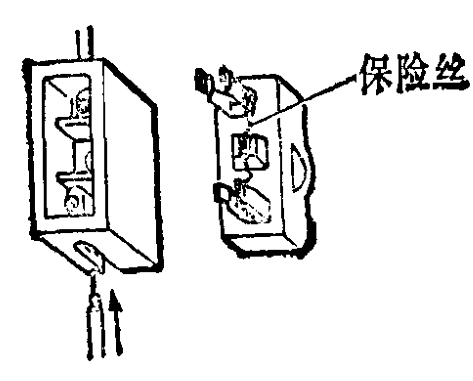
\includegraphics[width=6cm]{../pic/czwl2-ch11-6}
    \caption{插入式保险盒}\label{fig:11-6}
    \end{minipage}
    \qquad
    \begin{minipage}{7cm}
    \centering
    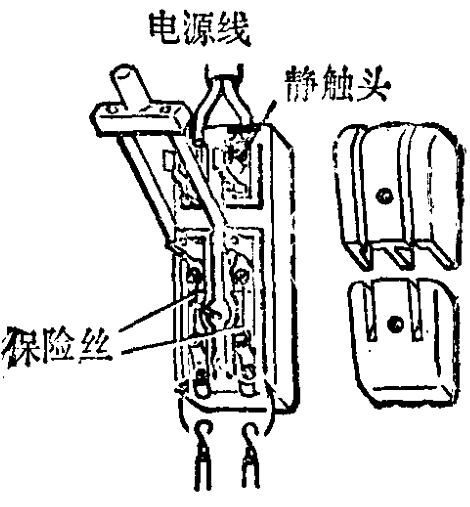
\includegraphics[width=6cm]{../pic/czwl2-ch11-7}
    \caption{闸刀开关}\label{fig:11-7}
    \end{minipage}
\end{figure}


\lianxi

(1) 找一个保险盒,打开盒盖,看看保险丝应该接在什么地方,然后练习一下装保险丝。

(2) 教室里装了 220 伏特、100 瓦特的电灯 6 盏,需要选用额定电流是多少安培的保险丝?

(3) 一座教学楼的总保险盒装的保险丝的额定电流是 25 安培,楼里共有 20 间教室,
每间教室装了 40 瓦特的电灯 6 盏。在全部电灯都亮着的时候,能否再接上一只 500 瓦特的电炉。

(4) 一台电烘箱,它的电热元件是由 4 条镍铬合金丝并联成的,每条镍铬合金丝的电阻都是 48.4 欧姆。
这台电烘箱将由照明电路供电。它的保险盒里应该装额定电流是多少安培的保险丝?

